\documentclass{beamer} % Использование класса beamer для создания презентации
\usetheme{Boadilla} % Применение темы Boadilla

\usepackage[T2A]{fontenc} % Установка кодировки шрифта
\usepackage[utf8]{inputenc} % Установка кодировки исходного текста
\usepackage[english,russian]{babel} % Подключение локализации и переносов для русского и английского языков
\usepackage{amsmath,amssymb} % Подключение математических символов и формул
\usepackage{autonum} % Автоматическая нумерация формул только при наличии ссылок на них
\usepackage{wrapfig} % Подключение пакета для обтекания текстом рисунков и таблиц
\usepackage{array} % Подключение пакета для работы с таблицами

\usepackage{tikz} % блок схема
\usetikzlibrary{shapes, arrows, positioning, calc}

\usepackage{graphicx}
\usepackage{amsmath}
\usepackage{booktabs}


\newcommand{\PreserveBackslash}[1]{\let\temp=\\#1\let\\=\temp} % Команда для сохранения обратной косой черты в ячейках таблицы
\newcolumntype{C}[1]{>{\PreserveBackslash\centering}p{#1}} % Создание нового типа столбца с центрированным содержимым

\usepackage[labelformat=empty]{caption} % Подключение пакета для настройки подписей и удаление названия "Рисунок"
\graphicspath{{./images/}{./images/logo/}} % Указание папок, где искать изображения

\setbeamertemplate{navigation symbols}{} % Удаление навигационных символов на слайдах
\usepackage{ragged2e} % Подключение пакета для улучшенного выравнивания текста
\newcommand{\jj}{\righthyphenmin=20 \justifying} % Команда для активации выравнивания по ширине с установкой минимального количества символов в слове перед переносом



\begin{document}




\begin{frame}
  \begin{center}\tiny
    Московский физико-технический институт (национальный исследовательский университет)\\
    Физтех-школа радиотехники и компьютерных технологий\\
    Кафедра микропроцессорных технологий в интеллектуальных системах управления
  \end{center}

  % \begin{center}
  %   \includegraphics[width=0.15\linewidth]{emb}
  % \end{center}

  \vspace{1 cm}
  \begin{center}\large
    % \textbf{КВАЛИФИКАЦИОННАЯ РАБОТА МАГИСТРА ТЕХНИКА И ТЕХНОЛОГИИ \\ ПО НАПРАВЛЕНИЮ 14040000.62 «ТЕХНИЧЕСКАЯ ФИЗИКА»}\\
    \vspace{0.2cm}
    % \textbf{НА ТЕМУ:}\\
    \vspace{0.1cm}
    \textbf{Реализация двухотсчетной следящей системы на основе вращающихся трансформаторов}
  \end{center}

  \vspace{2 cm}

  \begin{columns}
    \begin{column}{0.50\textwidth}
      \begin{center}\tiny
        Выполнил: \\
        \vspace{0.1cm}
        \textbf{Кутузов Виктор Михайлович}\\
        студент группы Б01-110 \\
      \end{center}
    \end{column}

    \begin{column}{0.50\textwidth}
      \begin{center}\tiny
        Научный руководитель:\\
        \vspace{0.1cm}
        \textbf{Какшин Виталий Витальевич} \\
        Ведущий инженер-исследователь
      \end{center}
    \end{column}
  \end{columns}

  \vspace{0.5cm}
  \begin{center}\tiny
    Москва, $2025$
  \end{center}
\end{frame}

\begin{frame}{План презентации}

\begin{itemize}
\item Актуальность
\item Цель
\item Техническое задание
\item Анализ датчиков
\item Аппаратная платформа
\item Программное обеспечение
% \item Алгоритм согласования двухотсчетной системы
\item Результаты испытаний
\item Заключение и практическая значимость
\end{itemize}
\end{frame}



\begin{frame}{Актуальность}

\begin{center}
  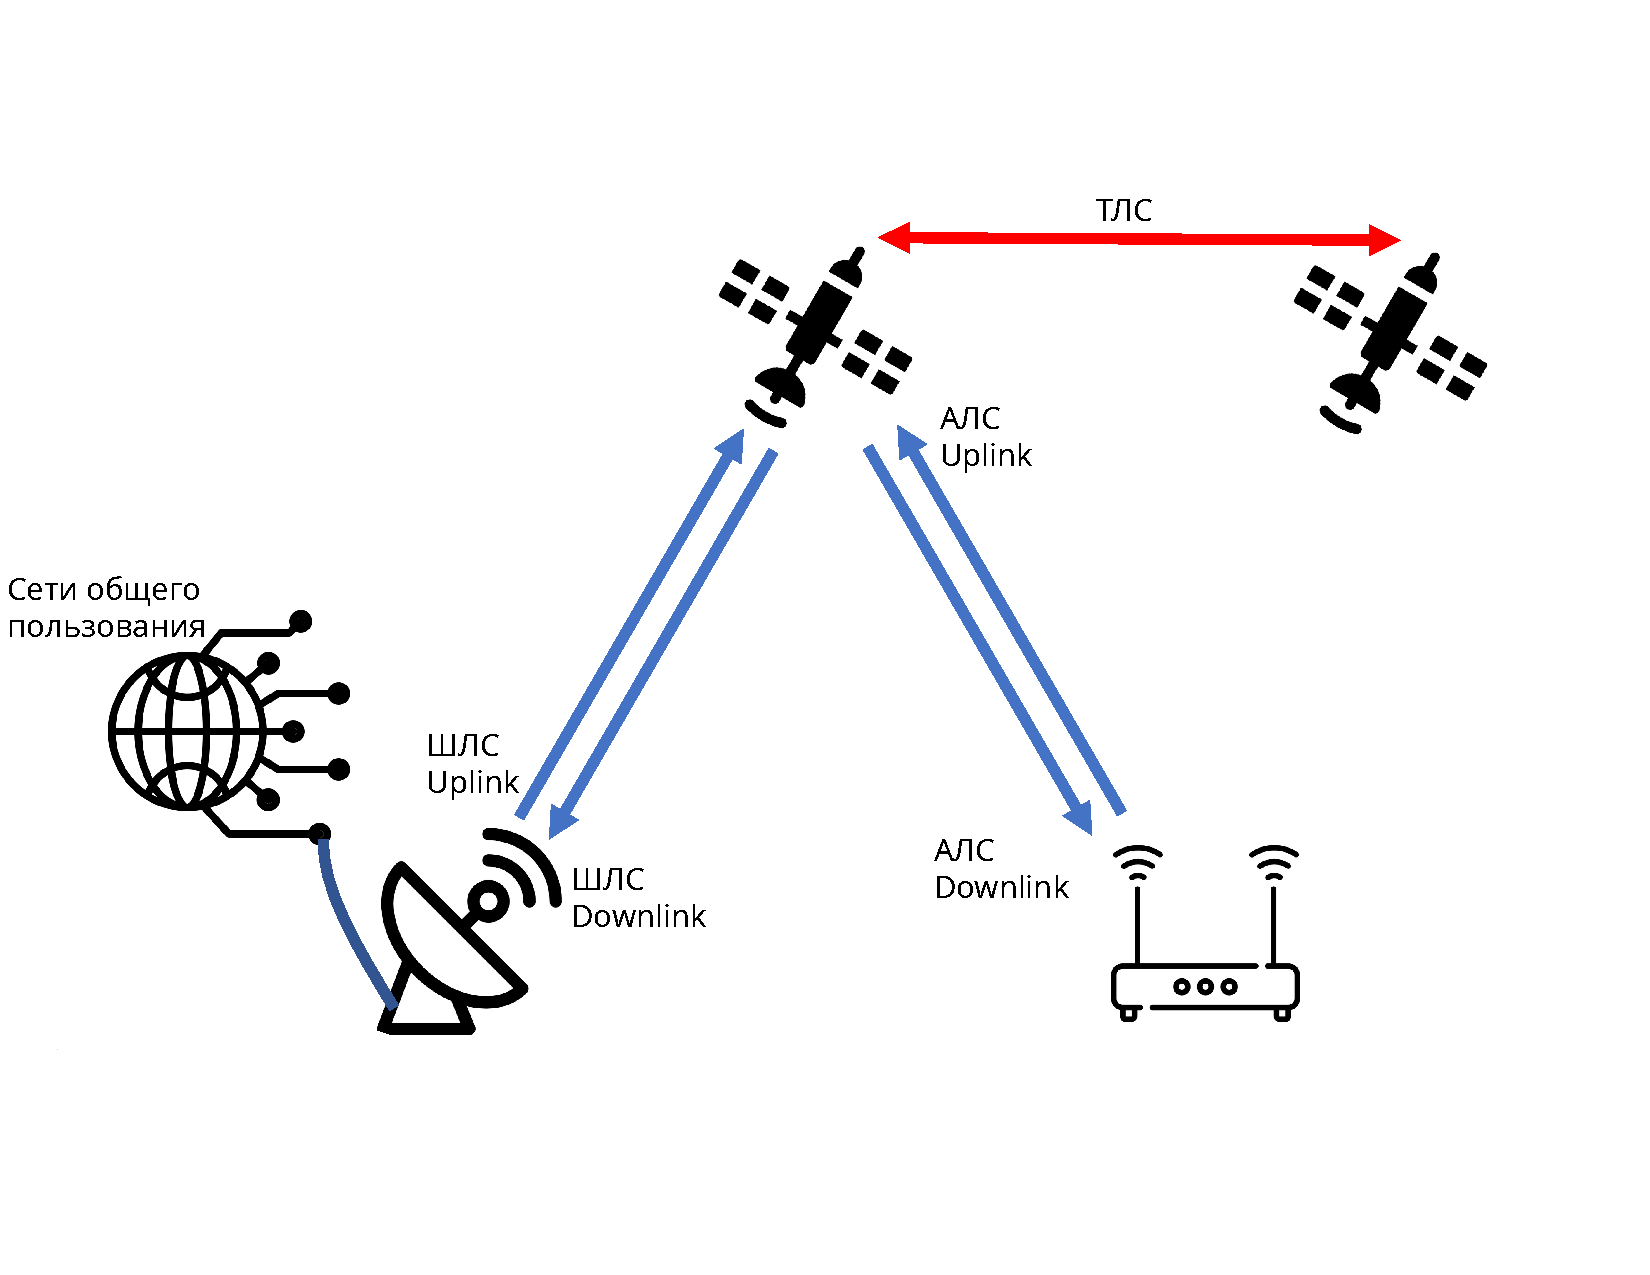
\includegraphics[height=0.65 \textheight,width=\textwidth,keepaspectratio=false]{SpaceSystem.pdf}
\end{center}

\begin{block}{}
\begin{itemize}\tiny
\item Необходимость глобального спутникового интернета
\item Низкоорбитальные группировки → высокоточное позиционирование антенн ( $ \pm 2'$, $\omega=30^\circ$/с)
\item Сложные условия эксплуатации
\end{itemize}
\end{block}
\end{frame}

\begin{frame}{Цель}

\begin{columns}
\column{0.5\textwidth}
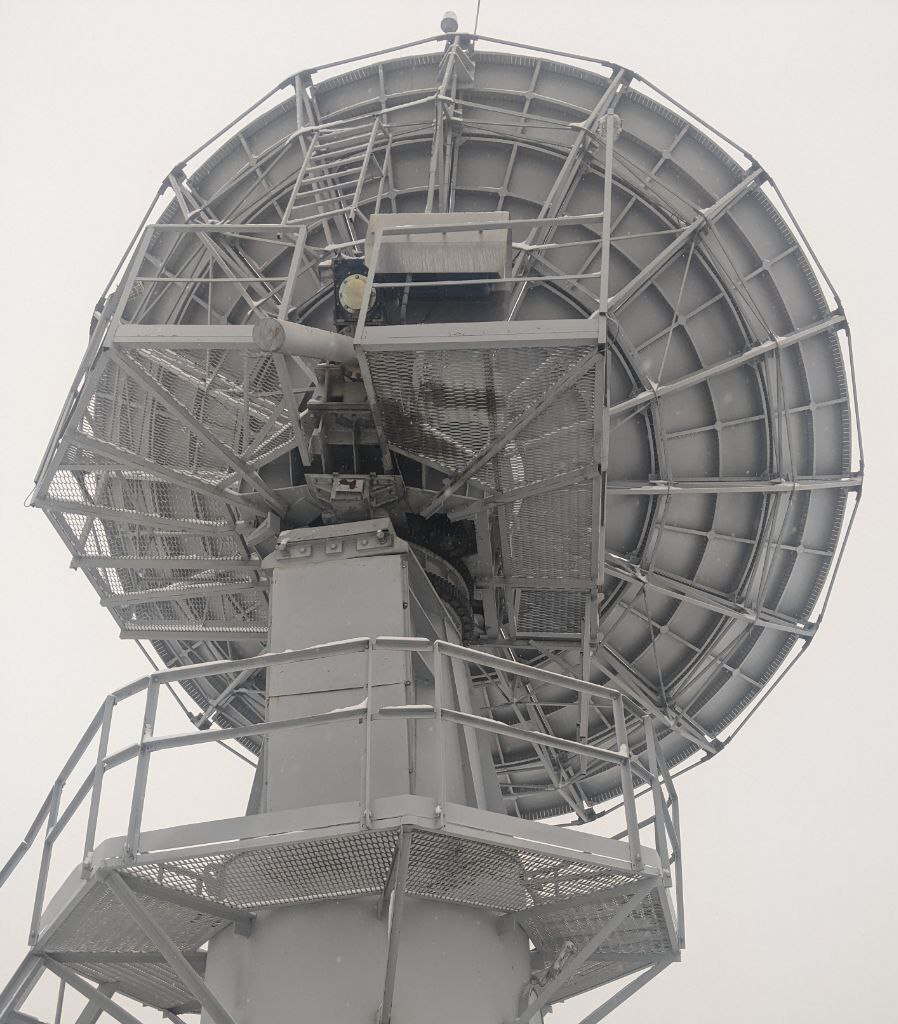
\includegraphics[width=\textwidth]{SnowAntenna.jpg}

\column{0.5\textwidth}
\begin{block}{}
Разработка и реализация программно-аппаратного комплекса для высокоточного (±2') 
измерения углового положения антенны
\end{block}

\end{columns}
\end{frame}

\begin{frame}{Техническое задание}
\centering
\begin{tabular}{lp{5cm}}
\toprule
Параметр & Требование \\
\midrule
Статическая погрешность & $\pm 2'$ \\
Динамическая ошибка & $\pm 2 '$ при $\omega \leq 30^\circ$/с \\
Частота обновления & $10$ кГц \\
Cопровождение & Непрерывное в течение сеанса связи \\
\bottomrule
\end{tabular}

\end{frame}


\begin{frame}{Анализ датчиков}
\centering
\begin{tabular}{lccc}
\toprule
Характеристика & Оптические & Магнитные & \textbf{ВТ} \\
\midrule
Точность & $ \leq 1'$ & $\approx 4'$ & \textbf{$\pm 2-5'$} \\
Темп. диапазон & $-10...+70^\circ C$ & $-20...+85^\circ C$ & \textbf{$-60...+150^\circ C$} \\
Влажность & Критична & Критична & \textbf{Устойчивы} \\
Надежность & Низкая & Средняя & \textbf{Высокая} \\
\bottomrule
\end{tabular}

\vspace{5mm}
\textbf{Выбранное решение:} \\
Вращающиеся трансформаторы ЛИР-ДР158А \\
в двухотсчетной схеме (редукция 1:36)

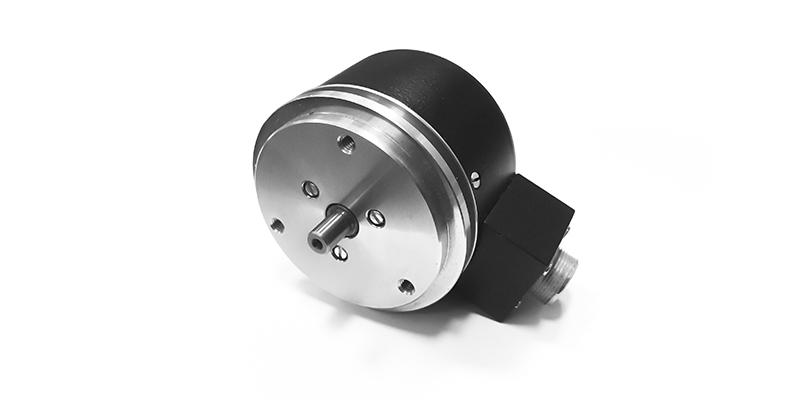
\includegraphics[width=0.6\textwidth]{ЛИР-ДР158A.jpg}
\end{frame}

\begin{frame}{Аппаратная платформа АЦПВТ}
\begin{figure}
  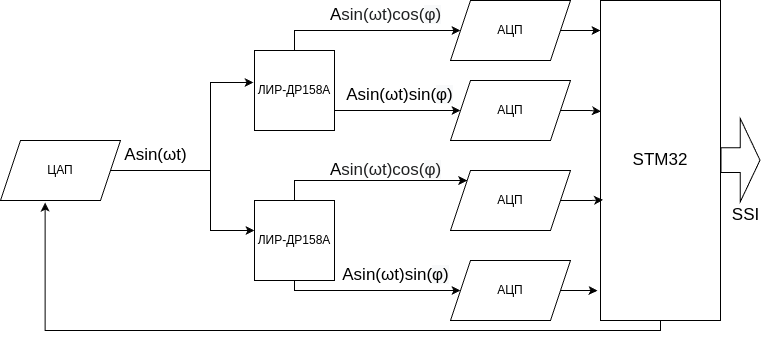
\includegraphics[width=\textwidth]{аппаратная_схема.png}
  \caption{Аппаратная реализация модуля}
\end{figure}
\end{frame}

% \begin{block}{Ключевые компоненты}
% \begin{itemize}
% \item Микроконтроллер: STM32F7 (Cortex-M7)
% \item Генерация возбуждения: ЦАП AD5331 → Усилители LM8261
% \item Оцифровка: 4× АЦП AD7492 (12-бит, 1.5 MSPS)
% \item Синхронизация: Каскад таймеров 
% \item Интерфейс: SSI (18 бит, код Грея, 100 кГц)
% \end{itemize}
% \end{block}

\begin{frame}{Аппаратная синхронизация таймеров}
\begin{figure}
  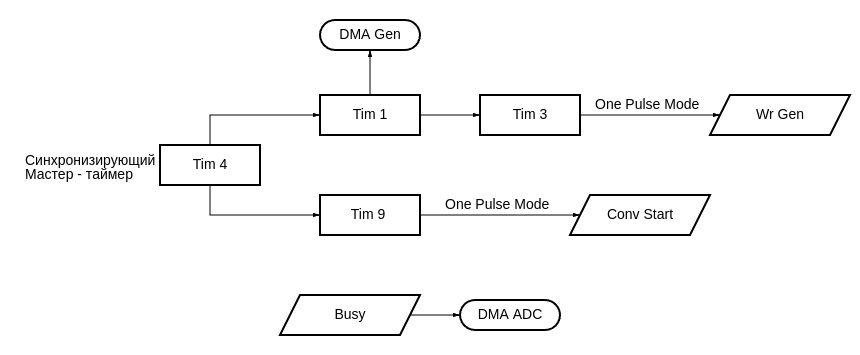
\includegraphics[width=\textwidth]{TimersScheme1.png}
  \caption{Схема синхронизации таймеров}
\end{figure}
\end{frame}

\begin{frame}{Взаимодействие с ВТ}
\begin{columns}
  \column{0.48\textwidth}
    \begin{figure}
      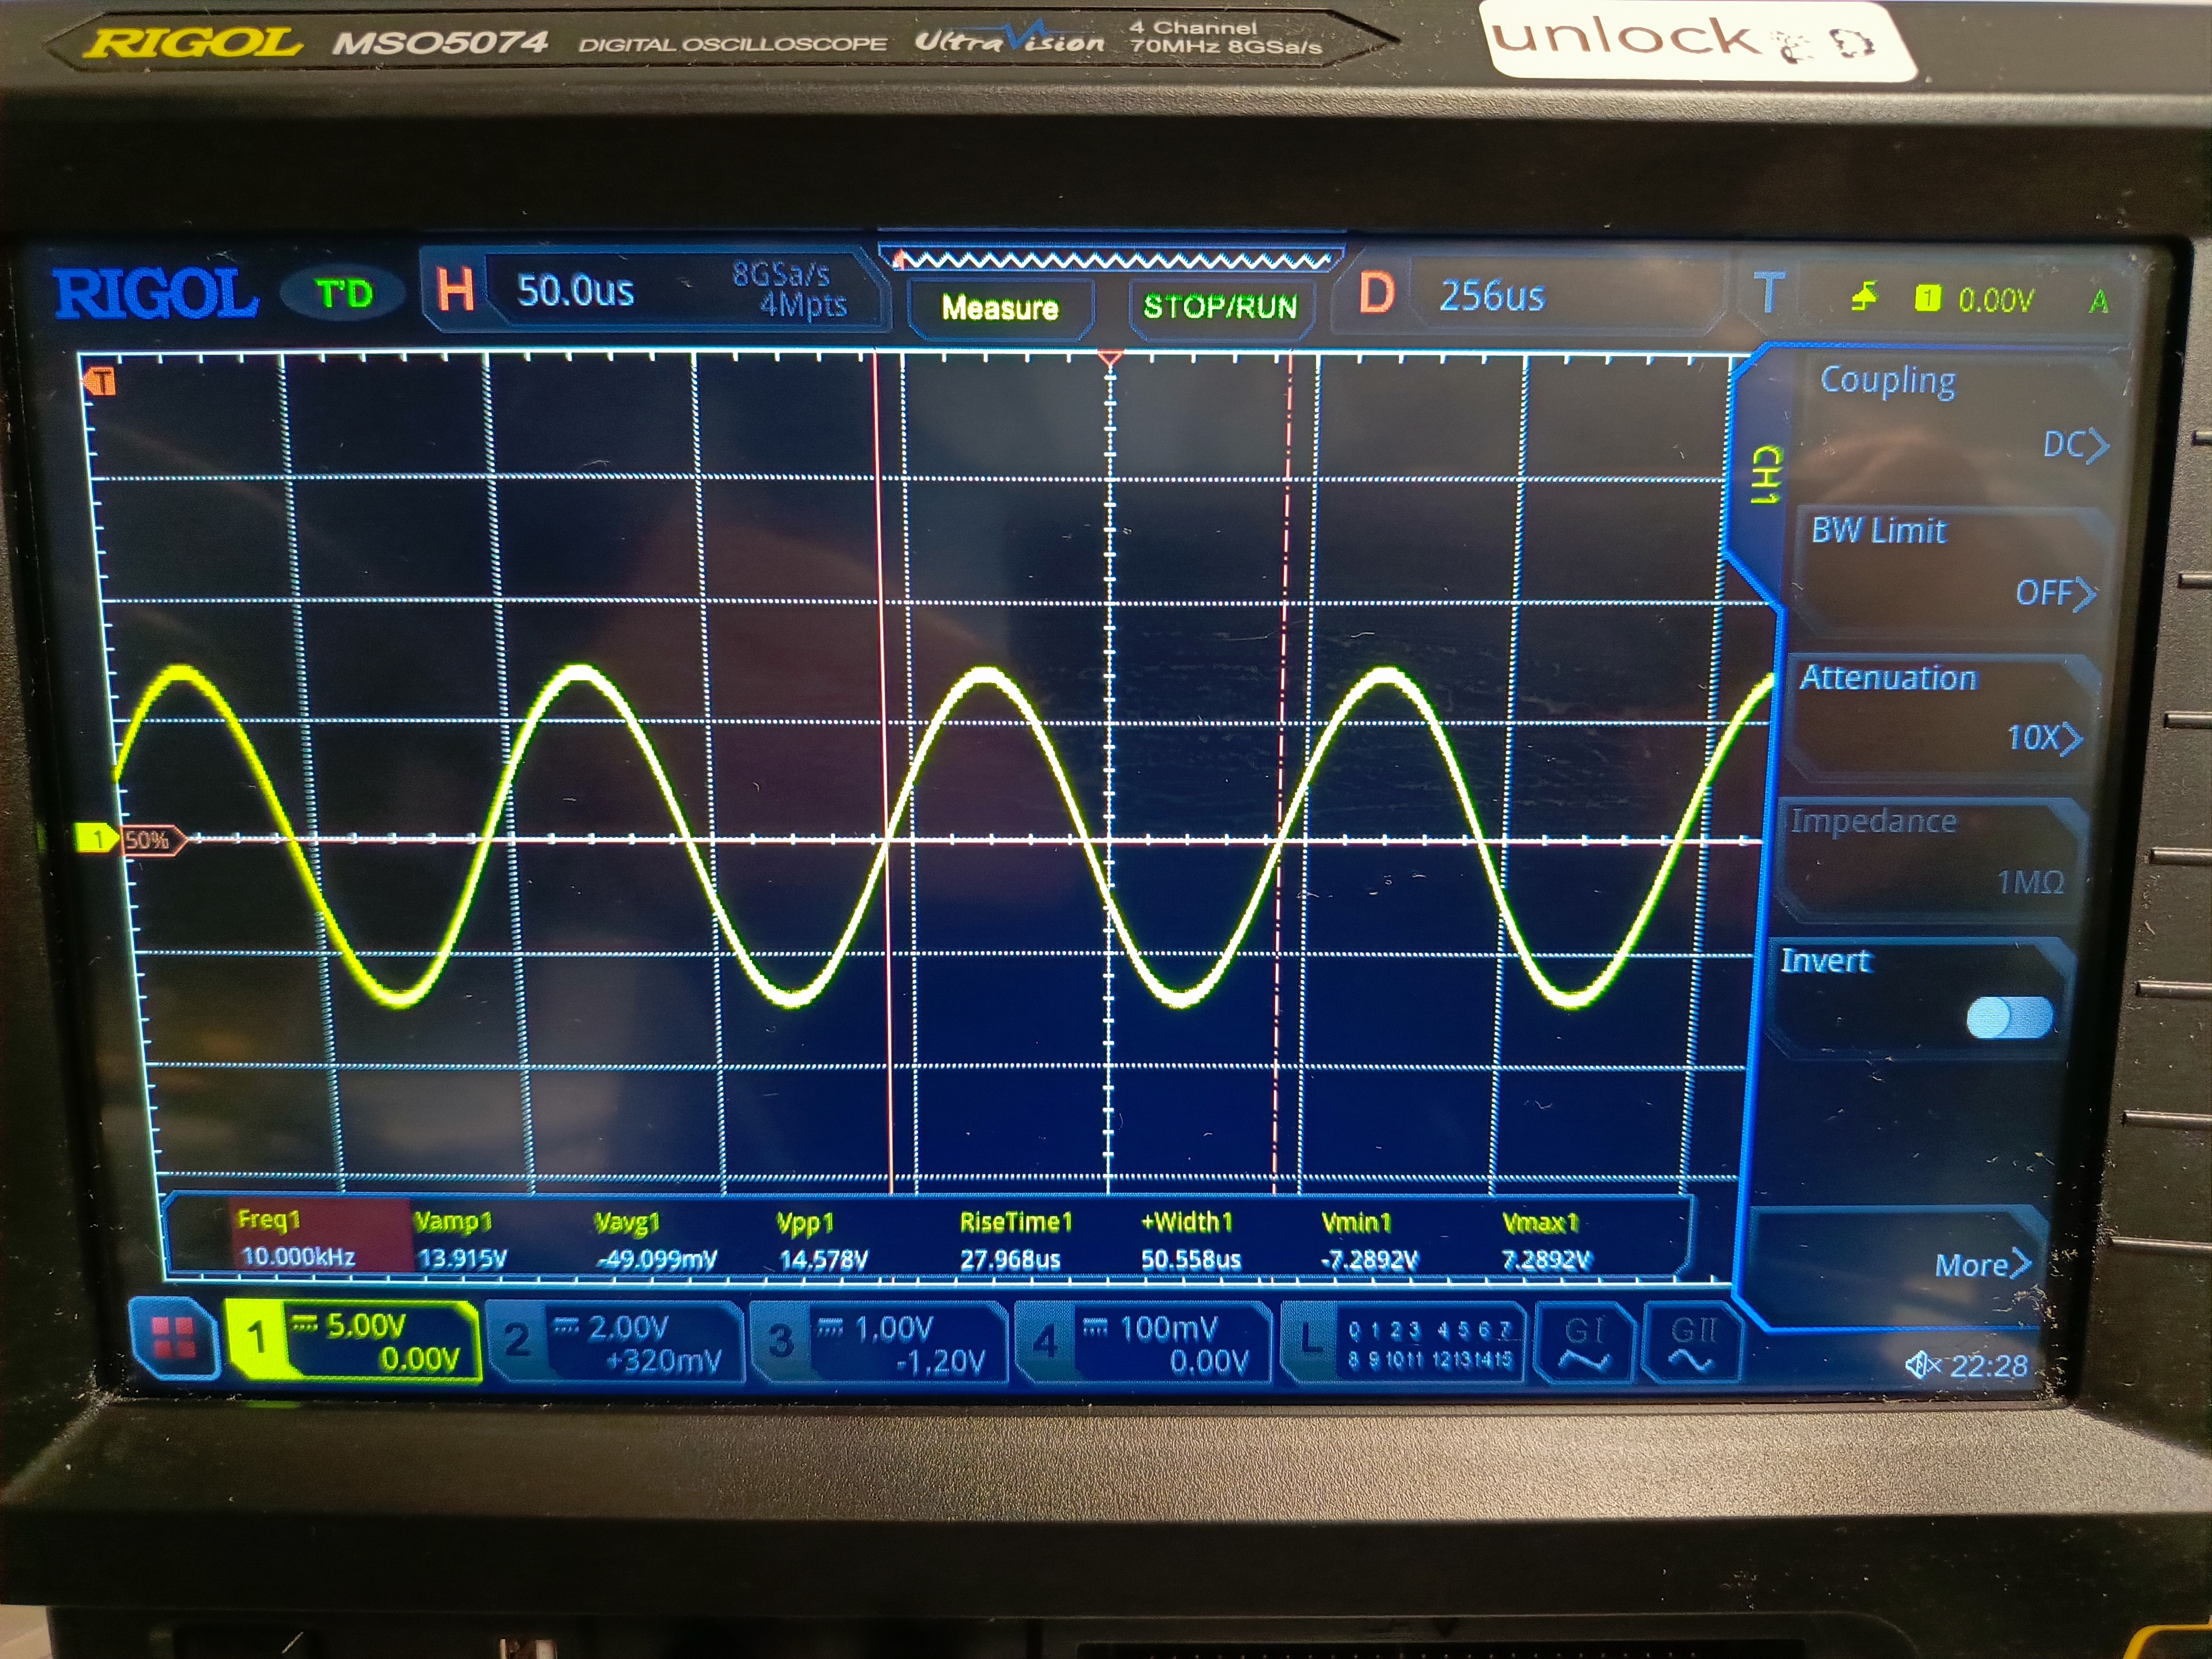
\includegraphics[width=\textwidth]{OSC_SIN.jpg}
      \caption{Сигнал на обмотке возбуждения}
    \end{figure}
  

 \column{0.48\textwidth}
    \begin{figure}
      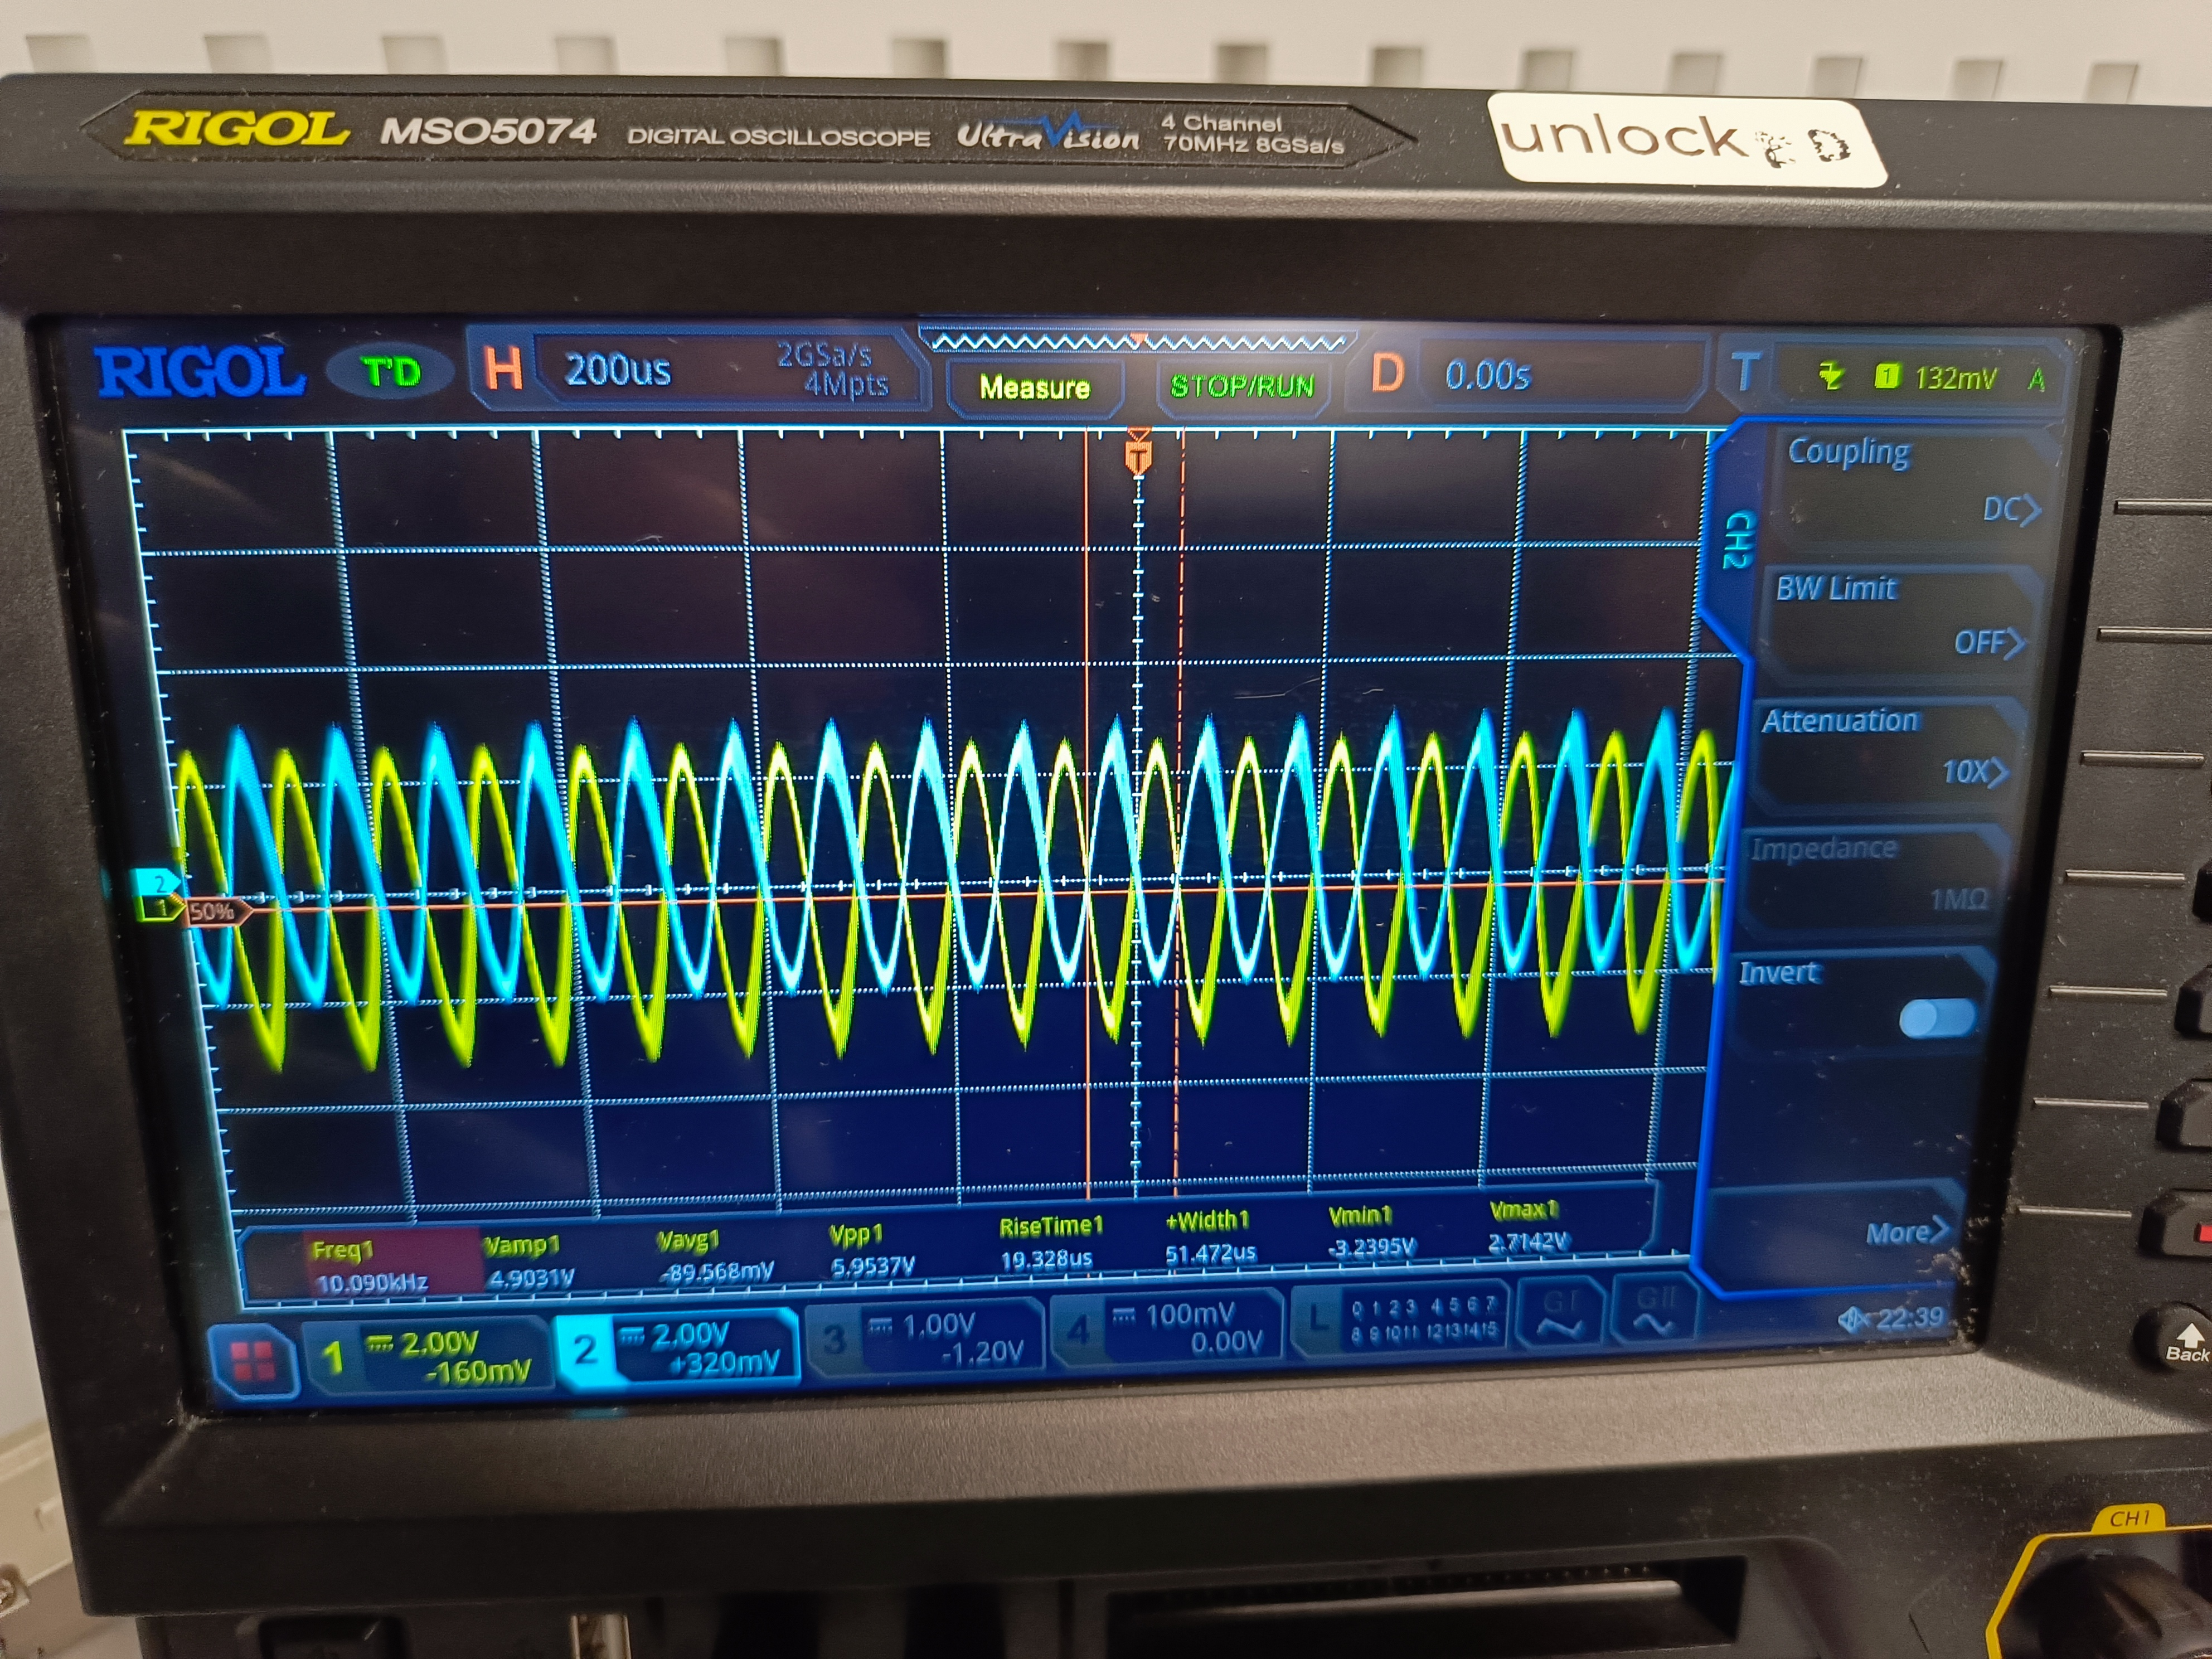
\includegraphics[width=\textwidth]{OSC_COS.jpg}
      \caption{Сигналы с вторичных обмоток  }
    \end{figure}
  
\end{columns}
\end{frame}

\begin{frame}{Алгоритм следящего преобразования}

% \column{0.5\textwidth}
\begin{figure}[ht]
  \resizebox{\textwidth}{!}{%
  \begin{tikzpicture}[
      block/.style={
          rectangle, 
          draw, 
          text width=6em, 
          text centered, 
          minimum height=3em, 
          font=\small,
          rounded corners=3pt
      },
      arrow/.style={->, thick, >=stealth},
      node distance=1.2cm and 0.8cm,
    ]
  
  % Блоки
  \node[block] (multSin) {Умножитель на $\cos(\phi')$};
  \node[block, below=of multSin] (multCos) {Умножитель на $\sin(\phi')$};
  \node[block, right=of multSin] (detector) {Детектор ошибки};
  \node[block, right=of detector] (integrator) {Интегратор угла};
  
  % Сигналы
  \node[left=of multSin] (inputSin) {$ V sin(\omega t) sin(\phi)$};
  \node[left=of multCos] (inputCos) {$ V sin(\omega t) cos(\phi)$};
  \node[right=of integrator] (output) {$\omega$};
  
  % Обратная связь: phi' к умножителям
  \coordinate (feedback) at ($(integrator.east)!0.5!(output.west)$);
  \node[above=0.3cm of feedback, font=\scriptsize] {};
  \draw[arrow, dashed, red] (integrator.north) -- ++(0.5cm,0) |- ([yshift=1cm]multSin.north) -- (multSin.north);
  \draw[arrow, dashed, red] (integrator.south) -- ++(0.5cm,0) |- (multCos.east); %([yshift=1cm]multCos.south) -- 
  
  % Основные соединения
  \draw[arrow] (inputSin) -- (multSin);
  \draw[arrow] (inputCos) -- (multCos);
  \draw[arrow] (multSin) -- (detector);
  \draw[arrow] (multCos) -- (detector);
  \draw[arrow] (detector) -- node[below=0.7cm] {} (integrator);
  \draw[arrow] (integrator) -- (output);
  
  % Пояснение обратной связи
  \node[above=0.1cm of multSin, align=center, font=\scriptsize] {};
  \node[below=0.1cm of multCos, align=center, font=\scriptsize] {Обратная связь: \\ $\phi'$ обновляется \\ через интегратор};
  
  \end{tikzpicture}
  } % Конец resizebox
  \caption{Схема следящего преобразователя с обратной связью} % Красные пунктирные линии показывают передачу оценки угла $\phi'$ обратно в умножители.
  \label{fig:tracking_scheme}
  
  \end{figure}
% \end{columns}
\end{frame}


% \begin{frame}[fragile]{Алгоритм следящего преобразования}
% % \begin{columns}
% % \column{0.5\textwidth}
% % \textbf{Математическая модель:}
% \begin{block}{Математическая модель:}
% \begin{itemize}


% \item $V_{sin} = V \sin(\omega t) \sin(\phi) $ 

% \item $V_{cos} = V \sin(\omega t) \cos(\phi) $ 

% \item $\varepsilon \approx V \sin(\omega t) (\phi - \phi') $ 

% \item $\phi'(t) = K_i \int_0^t \varepsilon(\tau) d\tau + \phi_0'$ 
% \end{itemize}
% \end{block}

% \begin{block}{Преимущества:}
% \begin{itemize}
% \item Нулевая статическая ошибка
% \item Разрешение до 19 бит
% \item Подавление помех
% \end{itemize}
% \end{block}

% \end{frame}



% \begin{frame}{Алгоритм согласования двухотсчетной системы}

% \begin{block}{Условие когерентности:}
% \[
% \left| \frac{\phi_r + 360^\circ \cdot i}{k_r} - \frac{\phi_T + 360^\circ \cdot n}{k_T} \right| \leq \Delta \phi
% \]
% \end{block}

% \begin{block}{Параметры:}
% \begin{itemize}
% \item $k_r = 1$ (грубый)
% \item $k_T = 36$ (точный)
% \item $\Delta \phi = \sqrt{\delta \phi_r^2 + \delta \phi_T^2}$
% \end{itemize}
% \end{block}

% \begin{block}{Результирующий угол:}

% \[
% N_\phi = \frac{\phi_T + 360^\circ \cdot n}{k_T}
% \]
% \end{block}

% \end{frame}

\begin{frame}{Алгоритм согласования двухотсчетной системы}

\begin{figure}[ht]
\resizebox{\textwidth}{!}{
\begin{tikzpicture}
    % Nodes
    \node (i_n)[draw, ellipse]  {i = 0; n = 0}; %[below of=phi]
    \node (check)[below of=i_n, yshift=-1cm][draw, rectangle]{ \( \left| \frac{(\phi_\text{г} + 360 \cdot i)}{k_\text{г}} - \frac{(\phi_\text{т} + 360 \cdot n)}{k_\text{т}} \right| \leq \Delta \phi?  \) }; %[below of=i_n]
    \node (phi_update) [right of=check, xshift=6cm][draw, rectangle] {\(\phi_\text{т} = \frac{\phi_\text{г} + 360 \cdot n}{k_\text{т}} \) };
    \node (n_less_kt) [below of=check, yshift=-1cm][draw, ellipse] {\( n < k_\text{т} ?\)};
    \node (n_increment) [left of=n_less_kt, xshift=-3cm] {\( n++\)};
    \node (i_less_kg) [below of = n_less_kt, yshift=-1cm] [draw, ellipse] {\( i < k_\text{г}\)};
    \node (i_increment) [left of=i_less_kg, xshift=-3cm] {\( i = i + 1; \newline n = 0\)};

    \node (legend) [below of=phi_update, yshift=-0.3cm] { \textbf{Обозначения:}};
    \node (1)[below of=legend, yshift=0.5cm]{\( \phi_\text{г} \) — угол грубого канала}; 
    \node (2) [below of=1, yshift=0.5cm]{\( \phi_\text{т} \) — угол точного канала}; 
    \node (3) [below of=2, yshift=0.5cm]{ \( k_\text{г}, k_\text{т} \) — коэффициенты редукции}; 
    \node (4) [below of=3, yshift=0.5cm]{\( \Delta\phi \) — допустимая погрешность }; 
    \node (5) [below of=4, yshift=0.5cm]{\( i, n \) — счётчики периодов}; 
        % 
        % 
        % };
    
    % % Arrowss
    \draw[->] (i_n) -- (check);
    \draw[->] (check) -- node[yshift=0.3cm] {Да} (phi_update);
    \draw[->] (check) -- node[xshift=0.7cm] {Нет}(n_less_kt);
    \draw[->] (n_less_kt) -- node[yshift=0.3cm] {Да} (n_increment);
    \draw[->] (n_less_kt) -- node[xshift=0.7cm] {Нет}(i_less_kg);
    \draw[->] (i_less_kg) -- (i_increment);
    \draw[->] (n_increment) -- (check);
    \draw[->] (i_increment) -- (check);
  
\end{tikzpicture}
} 
\caption{Схема cогласования датчиков} 
\label{fig:sogl_sch}  
\end{figure}

\end{frame}


% \begin{frame}{Экспериментальный стенд}
% \centering


% \begin{block}{Компоненты стенда}
% \begin{itemize}
% \item Блок АЦПВТ
% \item 2× ВТ ЛИР-ДР158А с редуктором 1:36
% \item Эталонный энкодер: Siemens 6FX2001-5HE (±0.01°)
% \item Электропривод: АИР56A4У3
% \item ПЛК: Siemens S7-1500
% \end{itemize}
% \end{block}
% \end{frame}

\begin{frame}{Экспериментальный стенд}
  \centering
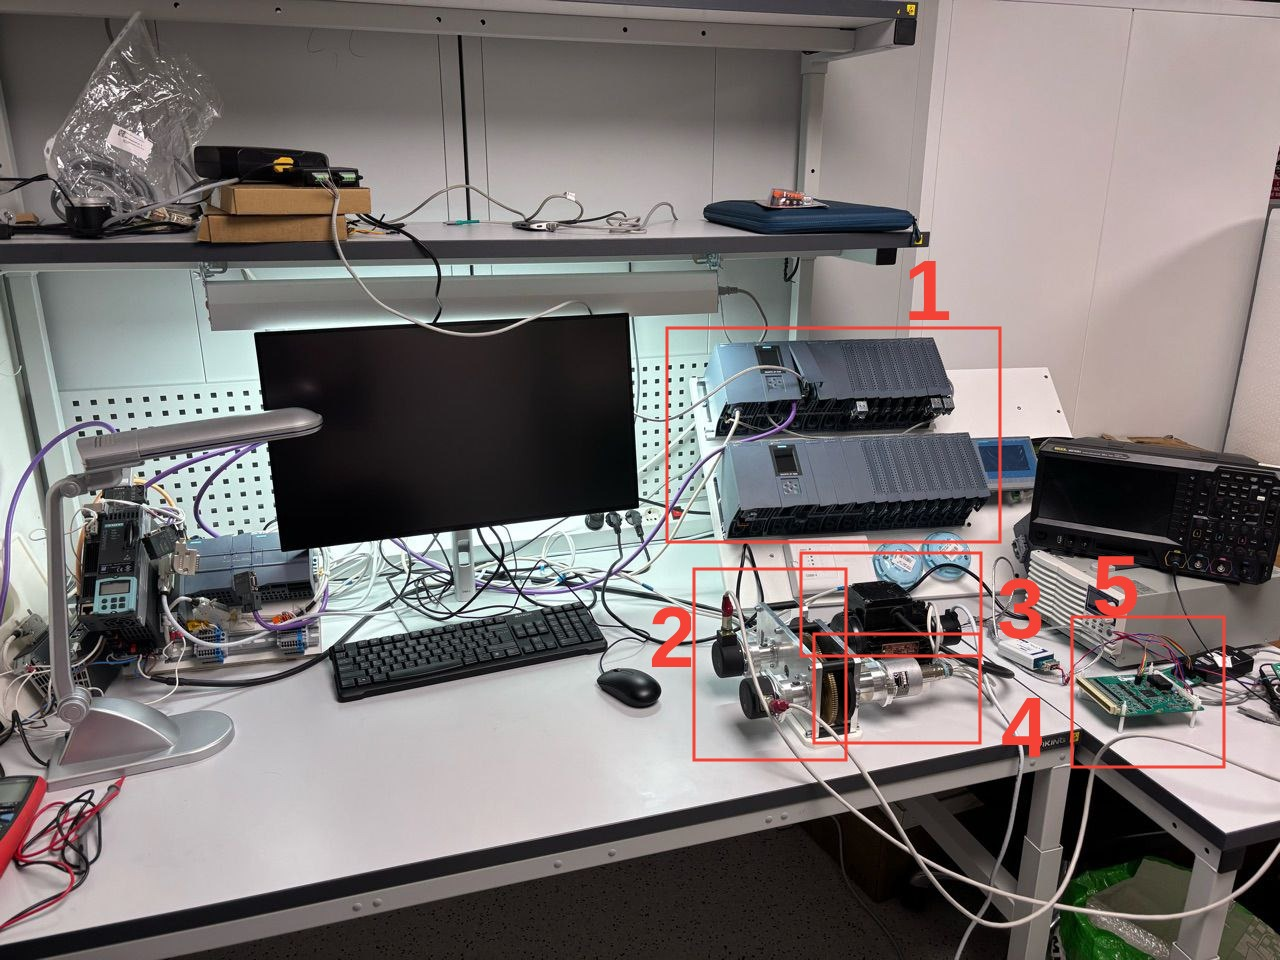
\includegraphics[width=\textwidth]{STND-02-comp.jpg}
\end{frame}

\begin{frame}{Структурная схема экспериментального стенда}
  \centering
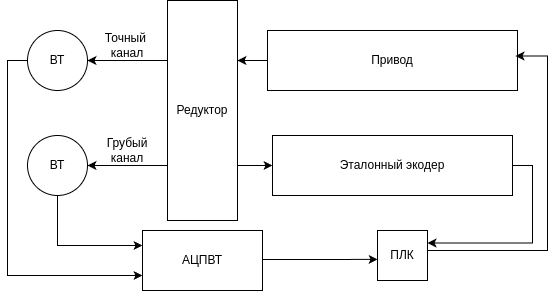
\includegraphics[width=\textwidth]{Test_Stand_SCH.png}
\end{frame}

\begin{frame}{Результаты испытаний}
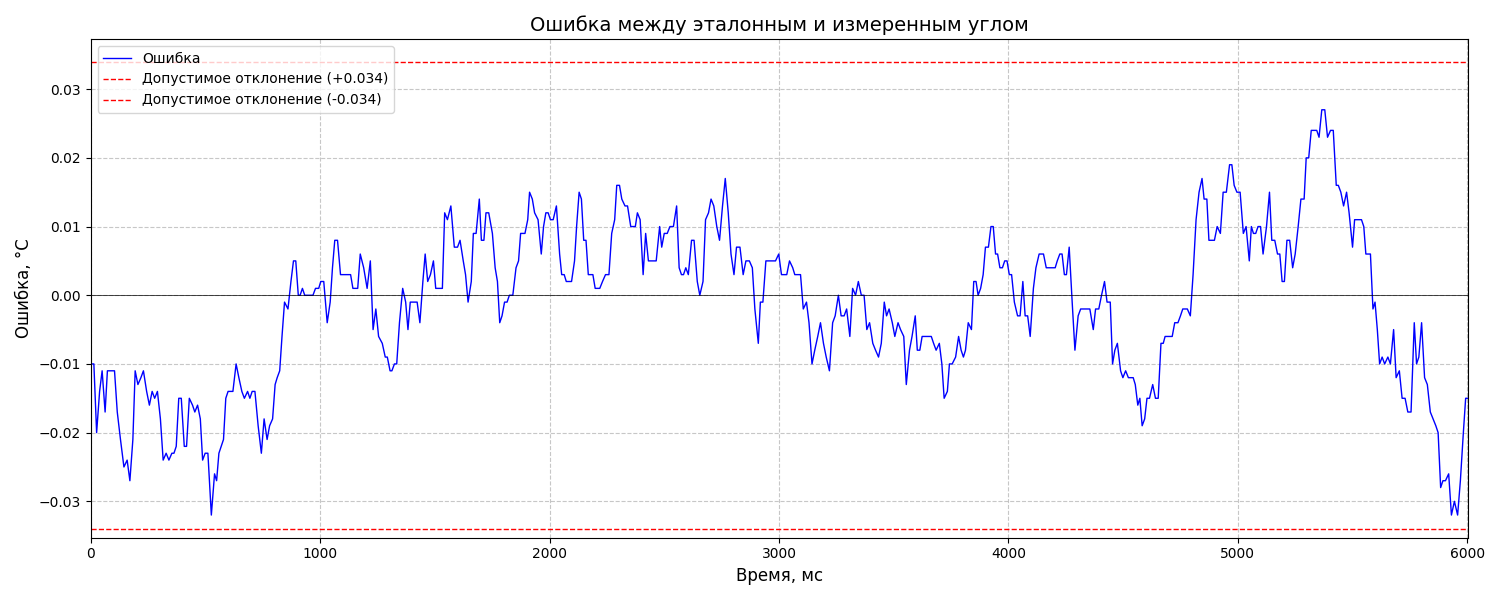
\includegraphics[width=\textwidth]{Figure_1.png}
\begin{block}{Достигнутые характеристики:}
\begin{itemize}
\item Динамическая ошибка: $< 2'$ при $\omega = 30^\circ$/с
\end{itemize}
\end{block}
\end{frame}

\begin{frame}{Заключение и практическая значимость}

\begin{block}{Ключевые результаты}
\begin{enumerate}
\item Обоснован выбор ВТ для экстремальных условий
\item Разработана архитектура АЦПВТ на STM32F7
\item Реализованы алгоритмы обработки сигналов
\item Экспериментально подтверждена точность
\end{enumerate}
\end{block}

% \textbf{Преимущества системы:}
% \begin{itemize}
% \item \textbf{Надежность}: ВТ вместо оптических энкодеров
% \item \textbf{Точность}: ±1' против ±5' у промышленных ВТ
% \item \textbf{Стоимость}: STM32 + Общепром. ВТ
% \item \textbf{Устойчивость}: Широкий климатический диапазон
% \end{itemize}

% \textbf{Перспективы:}
% \begin{itemize}
% \item Испытания при угловом ускорении
% \item Применение в робототехнике и ЧПУ
% \end{itemize}
\end{frame}

\begin{frame}
\begin{block}{Контактная информация}
\begin{itemize}
\item \textbf{Автор:} Кутузов Виктор Михайлович 
\item \textbf{Научный руководитель:} Какшин Виталий Витальевич
\item \textbf{Email:} kutuzov.vm@phystech.edu
\item \textbf{Телефон:} +7 987 169 55 04
\end{itemize}
\end{block}
\end{frame}


\end{document}
